% Options for packages loaded elsewhere
\PassOptionsToPackage{unicode}{hyperref}
\PassOptionsToPackage{hyphens}{url}
%
\documentclass[
  english,
  jou]{apa6}
\usepackage{lmodern}
\usepackage{amssymb,amsmath}
\usepackage{ifxetex,ifluatex}
\ifnum 0\ifxetex 1\fi\ifluatex 1\fi=0 % if pdftex
  \usepackage[T1]{fontenc}
  \usepackage[utf8]{inputenc}
  \usepackage{textcomp} % provide euro and other symbols
\else % if luatex or xetex
  \usepackage{unicode-math}
  \defaultfontfeatures{Scale=MatchLowercase}
  \defaultfontfeatures[\rmfamily]{Ligatures=TeX,Scale=1}
\fi
% Use upquote if available, for straight quotes in verbatim environments
\IfFileExists{upquote.sty}{\usepackage{upquote}}{}
\IfFileExists{microtype.sty}{% use microtype if available
  \usepackage[]{microtype}
  \UseMicrotypeSet[protrusion]{basicmath} % disable protrusion for tt fonts
}{}
\makeatletter
\@ifundefined{KOMAClassName}{% if non-KOMA class
  \IfFileExists{parskip.sty}{%
    \usepackage{parskip}
  }{% else
    \setlength{\parindent}{0pt}
    \setlength{\parskip}{6pt plus 2pt minus 1pt}}
}{% if KOMA class
  \KOMAoptions{parskip=half}}
\makeatother
\usepackage{xcolor}
\IfFileExists{xurl.sty}{\usepackage{xurl}}{} % add URL line breaks if available
\IfFileExists{bookmark.sty}{\usepackage{bookmark}}{\usepackage{hyperref}}
\hypersetup{
  pdftitle={Sans Forgetica is Not Desirable for Learning},
  pdflang={en-EN},
  pdfkeywords={Disfluency, Recall, Desirable Difficulty, Learning and Memory, Recognition},
  hidelinks,
  pdfcreator={LaTeX via pandoc}}
\urlstyle{same} % disable monospaced font for URLs
\usepackage{graphicx,grffile}
\makeatletter
\def\maxwidth{\ifdim\Gin@nat@width>\linewidth\linewidth\else\Gin@nat@width\fi}
\def\maxheight{\ifdim\Gin@nat@height>\textheight\textheight\else\Gin@nat@height\fi}
\makeatother
% Scale images if necessary, so that they will not overflow the page
% margins by default, and it is still possible to overwrite the defaults
% using explicit options in \includegraphics[width, height, ...]{}
\setkeys{Gin}{width=\maxwidth,height=\maxheight,keepaspectratio}
% Set default figure placement to htbp
\makeatletter
\def\fps@figure{htbp}
\makeatother
\setlength{\emergencystretch}{3em} % prevent overfull lines
\providecommand{\tightlist}{%
  \setlength{\itemsep}{0pt}\setlength{\parskip}{0pt}}
\setcounter{secnumdepth}{-\maxdimen} % remove section numbering
% Make \paragraph and \subparagraph free-standing
\ifx\paragraph\undefined\else
  \let\oldparagraph\paragraph
  \renewcommand{\paragraph}[1]{\oldparagraph{#1}\mbox{}}
\fi
\ifx\subparagraph\undefined\else
  \let\oldsubparagraph\subparagraph
  \renewcommand{\subparagraph}[1]{\oldsubparagraph{#1}\mbox{}}
\fi
% Manuscript styling
\usepackage{upgreek}
\captionsetup{font=singlespacing,justification=justified}

% Table formatting
\usepackage{longtable}
\usepackage{lscape}
% \usepackage[counterclockwise]{rotating}   % Landscape page setup for large tables
\usepackage{multirow}		% Table styling
\usepackage{tabularx}		% Control Column width
\usepackage[flushleft]{threeparttable}	% Allows for three part tables with a specified notes section
\usepackage{threeparttablex}            % Lets threeparttable work with longtable

% Create new environments so endfloat can handle them
% \newenvironment{ltable}
%   {\begin{landscape}\begin{center}\begin{threeparttable}}
%   {\end{threeparttable}\end{center}\end{landscape}}
\newenvironment{lltable}{\begin{landscape}\begin{center}\begin{ThreePartTable}}{\end{ThreePartTable}\end{center}\end{landscape}}

% Enables adjusting longtable caption width to table width
% Solution found at http://golatex.de/longtable-mit-caption-so-breit-wie-die-tabelle-t15767.html
\makeatletter
\newcommand\LastLTentrywidth{1em}
\newlength\longtablewidth
\setlength{\longtablewidth}{1in}
\newcommand{\getlongtablewidth}{\begingroup \ifcsname LT@\roman{LT@tables}\endcsname \global\longtablewidth=0pt \renewcommand{\LT@entry}[2]{\global\advance\longtablewidth by ##2\relax\gdef\LastLTentrywidth{##2}}\@nameuse{LT@\roman{LT@tables}} \fi \endgroup}

% \setlength{\parindent}{0.5in}
% \setlength{\parskip}{0pt plus 0pt minus 0pt}

% \usepackage{etoolbox}
\makeatletter
\patchcmd{\HyOrg@maketitle}
  {\section{\normalfont\normalsize\abstractname}}
  {\section*{\normalfont\normalsize\abstractname}}
  {}{\typeout{Failed to patch abstract.}}
\patchcmd{\HyOrg@maketitle}
  {\section{\protect\normalfont{\@title}}}
  {\section*{\protect\normalfont{\@title}}}
  {}{\typeout{Failed to patch title.}}
\makeatother
\shorttitle{Sans Forgetica}
\author{Jason Geller\textsuperscript{1}, Sara D. Davis\textsuperscript{2}, \& Daniel Peterson\textsuperscript{2}}
\affiliation{
\vspace{0.5cm}
\textsuperscript{1} University of Iowa\\\textsuperscript{2} Skidmore College}
\keywords{Disfluency, Recall, Desirable Difficulty, Learning and Memory, Recognition\newline\indent Word count: 5708}
\usepackage{dblfloatfix}


\usepackage{csquotes}
\ifxetex
  % Load polyglossia as late as possible: uses bidi with RTL langages (e.g. Hebrew, Arabic)
  \usepackage{polyglossia}
  \setmainlanguage[]{english}
\else
  \usepackage[shorthands=off,main=english]{babel}
\fi

\title{Sans Forgetica is Not Desirable for Learning}

\date{}

\abstract{
Do students learn better with material that is perceptually hard to process? While evidence is equivocal on the matter, recent claims suggest that placing materials in Sans Forgetica, a perceptually difficult-to-process typeface, has positive impacts on student learning. Given the weak evidence for other similar perceptual disfluency effects, we examined the mnemonic effects of Sans Forgetica more closely in comparison to other learning strategies across three preregistered experiments. In Experiment 1 (\emph{N} = 233), participants studied weakly related cue-target pairs with targets presented in either Sans Forgetica or with missing letters (e.g., cue: G\_RL, the generation effect). Cued recall performance showed a robust effect of generation, but no Sans Forgetica memory benefit. In Experiment 2 (\emph{N} = 528), participants read an educational passage about ground water with select sentences presented in either Sans Forgetica typeface, yellow pre-highlighting, or unmodified. Cued recall for select words was better for pre-highlighted information than a unmodified pure reading condition. Critically, presenting sentences in Sans Forgetica did not elevate cued recall compared to an unmodified pure reading condition or a pre-highlighted condition. In Experiment 3 (\emph{N} = 60), individuals did not have better discriminability for Sans Forgetica relative to a fluent condition in an old-new recognition test. Our findings suggest that Sans Forgetica really is forgettable.
}

% papaja Lua-filter additions

\authornote{

Funding Source: This research was supported by grant number 220020429 from the James S. McDonnell Foundation awarded to the third author.

Correspondence concerning this article should be addressed to Jason Geller, Department of Psychological and Brain Science, W113 Seashore Hall, Iowa City, IA, 52242. E-mail: \href{mailto:drjasongeller@gmail.com}{\nolinkurl{drjasongeller@gmail.com}}

}


\begin{document}
\maketitle

Students want to remember more and forget less. Being able to recall and apply previously learned information is key for successful academic performance at all levels. Many students are attracted to learning interventions that require minimal effort, but such approaches are rarely the best ways to achieve durable learning (Geller et al., 2018). Research in both the laboratory and classroom supports the paradoxical idea that making the encoding or retrieval of information more difficult, not easier, has the desirable effect of improving long-term retention (Bjork \& Bjork, 2011). Notable examples of desirable difficulties include the generation effect (improved memory for information that has been actively generated rather than passively read; Bertsch, Pesta, Wiscott, \& McDaniel, 2007; Slamecka \& Graf, 1978), and the testing effect (improved memory for information that was actively recalled rather than passively re-read; see Kornell \& Vaughn, 2016).

Research has conclusively established that when encoding is sufficiently effortful, memory outcomes improve. More recently, attention has focused on just how effortful that processing needs to be to observe mnemonic benefits. Specifically, researchers have examined whether subtle perceptual manipulations that change the physical characteristics of to-be-learned stimuli (rendering them harder to read or more disfluent) can similarly improve retention. Some research suggests it can. Diemand-Yauman, Oppenheimer, and Vaughan (2011), for instance, demonstrated that placing words in atypical typefaces (e.g., Comic Sans, Montype Corsiva) resulted in better memory than if the material was in a common typeface. A similar perceptual disfluency effect has been found with other perceptual manipulations including masking {[}e.g., presenting a stimulus very briefly (\textasciitilde100 ms) and forward or backing masking it; Mulligan (1996), inversion (Sungkhasettee, Friedman, \& Castel, 2011), blurring (Rosner, Davis, \& Milliken, 2015), and handwriting (Geller et al., 2018). The predominant theoretical explanation unifying these effects is that disfluency triggers metacognitive monitoring (\enquote{This is difficult to process}), which subsequently cues the learner to engage in deeper (i.e., more semantic) processing of material {[}but see Geller et al. (2018) for an alternative account).

Though this makes for a compelling story, other research casts serious doubt on disfluency as an effective pedagogical tool (e.g., Magreehan, Serra, Schwartz, \& Narciss, 2016; Rhodes \& Castel, 2008, p. @Rhodes2009; Rummer, Schweppe, \& Schwede, 2016; Yue, Castel, \& Bjork, 2013). A recent meta-analysis by Xie, Zhou, and Liu (2018) which included 25 studies and 3,135 participants found a small non-significant effect of perceptual disfluency on recall (\emph{d} = -0.01) and transfer (\emph{d} = 0.03). Most damning, despite having no mnemonic effect, perceptual disfluency manipulations generally produced longer reading times (\emph{d} = 0.52) and lower judgments of learning (JOLs) (\emph{d} = -0.43).

In trying to make sense of these disparate results, it is important to consider boundary conditions of the disfluency effect (see Geller \& Still, 2018; Geller et al., 2018). As Geller et al. (2018) argue, not all perceptual disfluency manipulations are created equal. In Geller et al. (2018), they compared memory outcomes for information that was presented in print or handwritten cursive that was either easy or hard-to-read. Results showed both easy and hard-to-read cursive were better remembered than print, but easy-to-read cursive was better remembered than hard-to-read cursive. This pattern suggests that disfluency manipulations can enhance memory, but such manipulations need to be optimally disfluent to exert a positive effect on memory.

Recently, a team of psychologists, graphic designers, and marketers set to create a new typeface specifically optimized to improve retention through perceptual disfluency. According to unpublished data from an interview taken from Earp (2018), to create the optimal typeface, the team conducted a cued recall experiment (\emph{N} = 96) wherein participants read 20 related word pairs (e.g., \emph{girl - guy}) each for 100 ms in a normal typeface (Albion) or one of three different disfluent typefaces (slightly disfluent, moderately disfluent, or extremely disfluent). They found an inverted U-shaped pattern wherein the moderately disfluent typeface was better remembered than the slightly and extremely disfluent typefaces. Further, they found that pairs in the moderately disfluent typeface were recalled slightly better than the normal typeface, although whether this meets the criteria for statistical significance is unclear. As a result of the memory boost, the team coined this moderately disfluent typeface Sans Forgetica. Sans Forgetica is a variant of sans serif typeface with intermittent gaps in letters that are back slanted (see Figure 1). The intermittent gaps of Sans Forgetica are thought to require readers to generate or fill in the missing pieces, thereby producing a memory advantage. This mechanism of action is thought to be similar to that of the generation effect, wherein information is better remembered when generated or filled in compared to if it is simply read (Slamecka \& Graf, 1978).

To examine the effects of Sans Forgetica under more educationally realistic conditions, the Sans Forgetica team presented participants (\emph{N} = 303) with 5 passages (\textasciitilde250 words in total) where one paragraph of three was presented in either the Sans Forgetica typeface or left in an unmodified (Arial) typeface (manipulated between subjects; Earp, 2018). For the Sans Forgetica condition, after each passage was read, participants were asked one question about the information written in the Sans Forgetica typeface and another question about the information written in Arial typeface. Performance was compared to the group that was presented with passages presneteed in a normal typeface. Placing text passages in the Sans Forgetica typeface resulted in better memory than if materials were presented in a normal typeface.

Since the release of the Sans Forgetica typeface, there has been a great deal of attention from the press. Sans Forgetica received coverage from major news sources like the Washington Post, National Public Radio, and The Guardian. In 2019, Sans Forgetica won the GoodDesign, Best in Class Award (Good Design, 2019). Commercially, Sans Forgetica typeface is freely available to users, and is marketed as a study tool Despite all the attention and marketing, empirical evidence for Sans Forgetica typeface is lacking.

Initial evidence for the Sans Forgetica typeface comes from the aforementioned unpublished studies by the Sans Forgetica development team (Earp, 2018). Note, however, that the modest group differences observed were not accompanied by any inferential hypothesis testing, nor were any of these claims subjected to the peer-review process. However, some evidence for the effectiveness of the Sans Forgetica typeface comes from a study by Eskenazi and Nix (2020), who found that words and definitions in Sans Forgetica typeface led to better orthographic discriminabity (i.e., choosing the correct spelling of a word) and semantic acquisition (i.e., retrieving the definition of a word), but only if participants were good spellers. This suggests that the utility of the Sans Forgetica typeface as a study tool may be quite limited. Recently, Taylor, Sanson, Burnell, Wade, and Garry (2020) found that although participants reported experiencing Sans Forgetica as disfluent (Experiment 1), there was no evidence that Sans Forgetica yielded a boost relative to Arial in cued recall (Expt 2) or for prose recall that tested factual (Experiment 3) and conceptual information (Experiment 4).

\hypertarget{the-present-studies}{%
\subsection{The Present Studies}\label{the-present-studies}}

The question of Sans Forgetica's effectiveness at producing a mnemonic benefit has clear educational implications. Demonstrating support for a purported study aid as quick and easy as swapping to-be-learned text from one typeface to another would be a boon for students. However, recent research calls into question the legitimacy of this typeface as a study aid at all (Taylor et al., 2020). Given the mixed evidence, the current set of studies aimed to further investigate the mnemonic benefit of the Sans Forgetica effect on memory.

In Experiment 1, we examined the impact of cue strength and study duration on cue-target pairs presented in a normal typeface or Sans Forgetica. In Experiment 2, we focused on more complex, educationally relevant prose passages. In Experiment 3, we examined if the type of test moderated the Sans Forgetica effect by using a yes/no recognition test. Importantly, we also compared the Sans Forgetica effect with other, more empirically supported learning techniques: generation (Experiment 1) and pre-highlighting (Experiment 2).

\hypertarget{experiment-1}{%
\section{Experiment 1}\label{experiment-1}}

In Experiment 1 we were interested in answering two questions. Does Sans Forgetica facilitate the retention of weakly associated cue-target pairs? If so, is this facilitation similar in magnitude to another desirable difficulty phenomenon---the generation effect? Taylor et al.~(Experiment 2) used cue-target pairs that were highly associated and failed to find a memory benefit for Sans Forgetica typeface. It has been argued (e.g.~Carpenter, 2009) that weakly related cue-target pairs produce more elaborative processing and lead to better memory, especially when the targets to be remembered require generation or retrieval (called the elaborative retrieval hypothesis). It is possible, then, that the use of highly associated pairs in Taylor et al. (2020) served to dampen the Sans Forgetica typeface effect. In Experiment 1 we examined the mnemonic benefit of Sans Forgetica typeface and generation by looking at cued recall performance with weakly associated cue-target pairs. In addition, we opted to present pairs for two seconds rather than the 100 ms duration used by Taylor et al. (2020) and Sans Forgetica team (Earp, 2018). With a 100 ms duration, participants might have struggled to read the word pairs properly, or to process the word pairs deeply enough, for any benefits of Sans Forgetica to take effect.

\hypertarget{method}{%
\subsection{Method}\label{method}}

Sample size, experimental design, hypotheses, outcome measures, and analysis plan for each experiment were pre-registered and can be found on the Open Science Framework (Experiments 1 and 2: \url{https://osf.io/d2vy8/}; Experiment 3: \url{https://osf.io/dsxrc/}). All raw and summary data, materials, and R scripts for preprocessing, analysis, and plotting can be found at \url{https://osf.io/d2vy8/}.

\hypertarget{participants}{%
\subsubsection{Participants}\label{participants}}

We recruited subjects on Amazon's Mechanical Turk (MTurk) platform, all of whom completed the study using Qualtrics survey software. A total of 232 people completed the experiment in return for U.S.\$1.00. Sample size was based on a priori power analyses conducted using PANGEA v0.2 (Westfall (2016)). Sample size was calculated based on the smallest effect of interest (SEOI; Lakens \& Evers, 2014). In this case, we were interested in powering our study to detect a medium sized interaction effect between the generation effect and the Sans Forgettica effect (\emph{d} = 0.35). We choose this effect size as our SESOI due in part to the small effect sizes seen in actual classroom studies (Butler, Marsh, Slavinsky, \& Baraniuk, 2014). Therefore, assuming an alpha of .05 and a desired power of 90\%, a sample size of 230 is required to detect whether an interaction effect size of 0.35 differs from zero. No participants met our pre-registered exclusion criteria (i.e., did not complete the experiment, started the experiment multiple times, experienced technical problems, or reported familiarity with the stimuli), yielding 116 participants in each between-subjects condition.

\hypertarget{design}{%
\subsubsection{Design}\label{design}}

Fluency (Fluent vs.~Disfluent) was manipulated within subjects and Disfluency Type (Generation vs.~Sans Forgetica) was manipulated between subjects. For the Sans Forgetica group, disfluent targets were presented in Sans Forgetica typeface while fluent targets were presented in Arial typeface. In the generation group, disfluent targets were presented in Arial typeface with missing letters (vowels replaced by underscores) and fluent targets were intact. See Figure 1 for an example of the stimuli used.

\begin{figure}

{\centering 
\includegraphics{/Users/gellr/SF_Expt/Picture1} 

}

\caption{Example of cue-target pairs. Left: Sans Forgetica condition. Right: Generation condition.Sans Forgetica is licensed under the Creative Commons Attribution-NonCommercial License (CC BY-NC; https:// creativecommons.org/licenses/by-nc/3.0/)}\label{fig:unnamed-chunk-1}
\end{figure}

\hypertarget{materials-and-procedure}{%
\subsubsection{Materials and Procedure}\label{materials-and-procedure}}

Participants were presented with 22 weakly related cue-target pairs taken from Carpenter et al.~(2006). The pairs were all nouns, 5--7 letters and 1--3 syllables in length, high in concreteness (400--700), high in frequency (at least 30 per million), and had similar forward (\emph{M} = 0.031) and backward (\emph{M} = 0.033) association strengths. Two counterbalanced lists were created for each Disfluency Type (Generation and Sans Forgetica) so that each item could be presented in each fluency condition without repeating any items for an individual participant.

Participants were randomly assigned to one of two conditions: the generation condition or the Sans Forgetica condition. Prior to studying the pairs, participants were instructed to mentally \enquote{fill in} the targets to come up with the correct target. Participants were also told to study word pairs so that later they could recall the target when presented with the cue. The experiment began with the presentation of the word pairs, presented one at a time, for five seconds each. After a short two-minute distraction task (anagram generation), participants completed a self-paced cued recall test. During cued recall, participants were presented 22 cues, one at a time, and asked to type in the target word. A short demographics survey followed this final test, after which participants were debriefed.

\hypertarget{scoring}{%
\subsubsection{Scoring}\label{scoring}}

Spell checking was automated with the hunspell package in R (Ooms, 2018). Using this package, each response was corrected for misspellings. Corrected spellings are provided in the most probable order; therefore, the first suggestion was always selected as the correct answer. As a second pass, we manually examined the output to catch incorrect suggestions. If the response was close to the correct response, it was marked as correct.

\hypertarget{analytic-strategy}{%
\subsubsection{Analytic Strategy}\label{analytic-strategy}}

For all the experiments, an alpha level of .05 is maintained. Cohen's d and generalized eta-squared (\(\eta_{g}^{2}\)\}; Olejnik \& Algina, 2003) are used as effect size measures. Alongside traditional analyses that utilize null hypothesis significance testing (NHST), we also report the Bayes factors for each analysis. All prior probabilities are Cauchy distributions centered at zero, and effect sizes are specified through the r-scale, which is the interquartile range (i.e., how spread out the middle 50\% of the distribution is). For the null model, the prior is set to zero. All data were analyzed in R (vers. 3.5.0; R Core Team, 2019), with models fit using the afex (vers. 0.27-2; Singmann et al., 2020) and BayesFactor packages (vers. 0.9.12-4.2; Morey \& Rouder, 2018). All figures were generated using ggplot2 (vers. 3.3.0; Wickham, 2006).

\hypertarget{results-and-discussion}{%
\section{Results and Discussion}\label{results-and-discussion}}

Per our pregreistation, cued recall accuracy was analyzed with a 2 (Fluency: Fluent vs.~Disfluent) x 2 (Disfluency Type: Generation vs.~Sans Forgetica) Mixed ANOVA. There was no difference in cued recall between the Generation and Sans Forgetica groups, \emph{F}(1, 230) = 0.19, \(\eta_{g}^{2}\) \textless.001, p = .752. Individuals recalled more disfluent target words than fluency target words, \emph{F}(1, 230) = 25.31, \(\eta_{g}^{2}\) =.017, \emph{p} \textless{} .001. This was qualified by an interaction between Fluency and Difficulty Type, \emph{F}(1, 230) = 25.06, \(\eta_{g}^{2}\) = .017, \emph{p} \textless{} .001. A Bayesian ANOVA indicated strong evidence for the interaction model over the main effects model, BF\textsubscript{10} \textgreater{} 100. As seen in Figure 2, the magnitude of the generation effect was larger than the Sans Forgetica effect, which was, in fact, negligible.

\begin{figure}
\centering
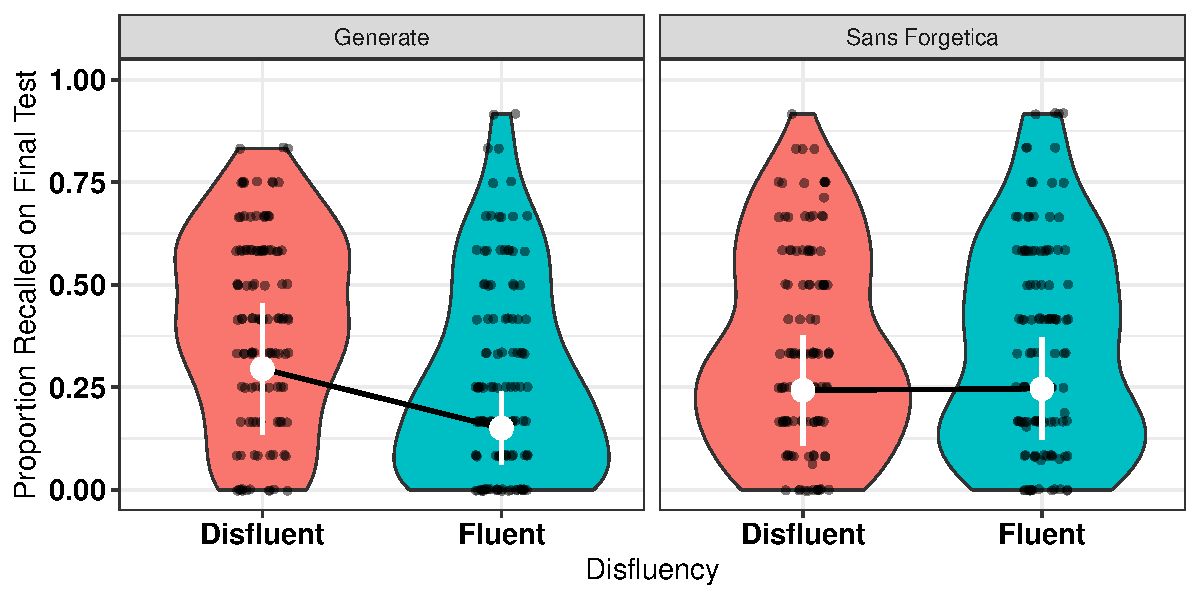
\includegraphics{SF_Paper_1_files/figure-latex/unnamed-chunk-2-1.pdf}
\caption{\label{fig:unnamed-chunk-2}Accuracy on cued recall test. Violin plots represent the kernal density of avearge accuracy (black dots) with the mean (white dot) and Cousineau-Morey within-subject 95\% CIs.}
\end{figure}

While the benefit of generating information was clear, there was no benefit of studying items in the Sans Forgetica typeface. Thus, presenting weakly associated targets in Sans Forgetica for two seconds produced no memory benefit. This null result was confirmed by a Bayesian analysis denoting strong evidence for the presence of the interaction compared to a main effects model. Although participants' overall accuracy was low in the current experiment (38\%), it is important to note that the level of performance was comparable to what was observed by Carpenter, Pashler, and Vul (2006) using the same materials (30\% overall for restudy compared to tested trials). In addition, accuracy was comparable to Experiment 2 from Taylor et al. (2020) who used highly associated cue target pairs (\textasciitilde45\%). Finally, overall performance was strong enough to reveal a significant generation effect, minimizing concerns that a difficult task might be suppressing an otherwise robust effect of Sans Forgettica . Taken together, these results suggest that (1) presenting materials in Sans Forgetica does not lead to better memory and (2) the effect of Sans Forgetica on memory is most likely not a desirable difficulty.

\hypertarget{experiment-2}{%
\section{Experiment 2}\label{experiment-2}}

Experiment 1 failed to reveal a memory benefit for the Sans Forgetica typeface. One potential limitation is that the atomistic stimuli employed in Experiment 1 (cue-target word pairs) may not provide an ecologically valid lens under which to study real classroom learning. To address this, in Experiment 2, we examined the mnemonic effects of Sans Forgetica using more complex prose materials. Like before, we wanted to compare the (potential) benefits of Sans Forgetica to something with empirical scrutiny. Accordingly, in Experiment 2, we examined how Sans Forgetica stacked up against pre-highlighting.

One of the purported functions of the Sans Forgetica typeface is to call attention to information one needs to remember. This is functionally similar to pre-highlighting, whereby important study information is highlighted prior to studying. Pre-highlighting is often used by instructors and textbook creators to enhance learning. Indeed, when students read pre-highlighted passages, there is some evidence that they recall more of the highlighted information and less of the non-highlighted information when compared to students who receive an unmarked copy of the same passage (Fowler \& Barker, 1974; Silvers \& Kreiner, 1997). To this end, Experiment 2 compared cued recall performance on a prose passage where some of the sentences were either presented in Sans Forgetica, pre-highlighted in yellow, or unmodified text. We hypothesized that both Sans Forgetica and pre-highlighting should enhance memory for selected passages compared to an unmodified passage.

\hypertarget{method-1}{%
\subsection{Method}\label{method-1}}

\hypertarget{participants-1}{%
\subsubsection{Participants}\label{participants-1}}

We preregistered a sample size of 510 (170 per group). When initial data collection finished, 683 participants participated for partial completion of course credit. After excluding participants based on our reregistered exclusion criteria (see above), we were left with unequal group sizes. Because of this, we ran six more participants per group, giving us 528 participants---176 participants in each of the three conditions.

\hypertarget{materials}{%
\subsubsection{Materials}\label{materials}}

Participants read a passage on ground water (856 words) taken from the U.S. Geological Survey (see Yue et al., 2014). Eleven critical phrases, each containing a different keyword, were selected from the passage (e.g., the term recharge was the keyword in the phrase \enquote{Water seeping down from the land surface adds to the ground water and is called recharge water}) and were presented in yellow (pre-highlighted), Sans Forgetica typeface, or unmodified typeface. Then, 11 fill-in-the blank questions were created from these phrases by deleting the keyword and asking participants to provide it on the final test (e.g., Water seeping down from the land surface adds to the ground water and is called \_\_\_\_\_\_\_\_\_\_ water). There was one attention check question at the beginning of the final test.

\hypertarget{design-and-procedure}{%
\subsubsection{Design and Procedure}\label{design-and-procedure}}

Participants completed the experiment online via the Qualtrics survey platform. Participants were randomly assigned to one of three conditions: pre-highlighting, Sans Forgetica, or unmodified text. Participants read a passage on ground water. All participants were instructed to read the passage as though they were studying material for a class. After 10 minutes, all participants were given a question asking them to provide a judgement of learning after reading the passage: \enquote{How likely is it that you will be able to recall material from the passage you just read on a scale of 0 (not likely to recall) to 100 (likely to recall) in 5 minutes?} Participants were then given a short distraction task (anagrams) for three minutes. Finally, all participants were given 11 fill-in-the-blank test questions, presented one at a time.

\hypertarget{scoring-1}{%
\subsubsection{Scoring}\label{scoring-1}}

Spell checking was automated with the same procedure as Experiment 1.

\hypertarget{results-and-discussion-1}{%
\subsection{Results and Discussion}\label{results-and-discussion-1}}

Per our preregistration, cued recall accuracy was analyzed with a one-way ANOVA (Passage Type: Pre-highlighting vs.~Sans Forgetica vs.~Unmodified). The one-way ANOVA was significant, F(2, 525) = 3.16, \(\eta_{g}^{2}\) = .012, \emph{p} = .043. We hypothesized that pre-highlighted and Sans Forgetica sentences would be better remembered than normal sentences and that there would be no recall differences in recall between the highlighted and Sans Forgetica sentences. Our hypotheses were partially supported (see Figure 3). Examining our planned comparisons, we found that pre-highlighted sentences were better remembered than sentences presented in unformatted text, \emph{t}(525) = 2.45, \emph{SE} = 0.028, \emph{p}\textsubscript{tuk} = .039, \emph{d} = 0.26. There was weak evidence for no effect between sentences presented in Sans Forgetica and pre-highlighted, \emph{t}(525) = 0.049, \emph{SE} = 0.028, \emph{p}\textsubscript{tuk} = .202, \emph{d} = 0.18, BF\textsubscript{01} = 2.36. Critically, there was no difference between sentences presented normally or in Sans Forgetica, \emph{t}(525) = 0.02, \emph{SE} = 0.028, \emph{p}\textsubscript{tuk} = .734, \emph{d} = 0.079, BF\textsubscript{01} = 6.47.

In short, we did not find that select information presented in Sans Forgetica produced better memory than select information left unmodified or pre-highlighted. The finding that Sans Forgetica typeface does not enhance memory for prose passages replicates the findings of Taylor et al. (2020) (Experiments 3 and 4). We did, however, observe better memory for pre-highlighted information compared to words presented unmodified or in a Sans Forgetica typeface.

\begin{figure}

{\centering 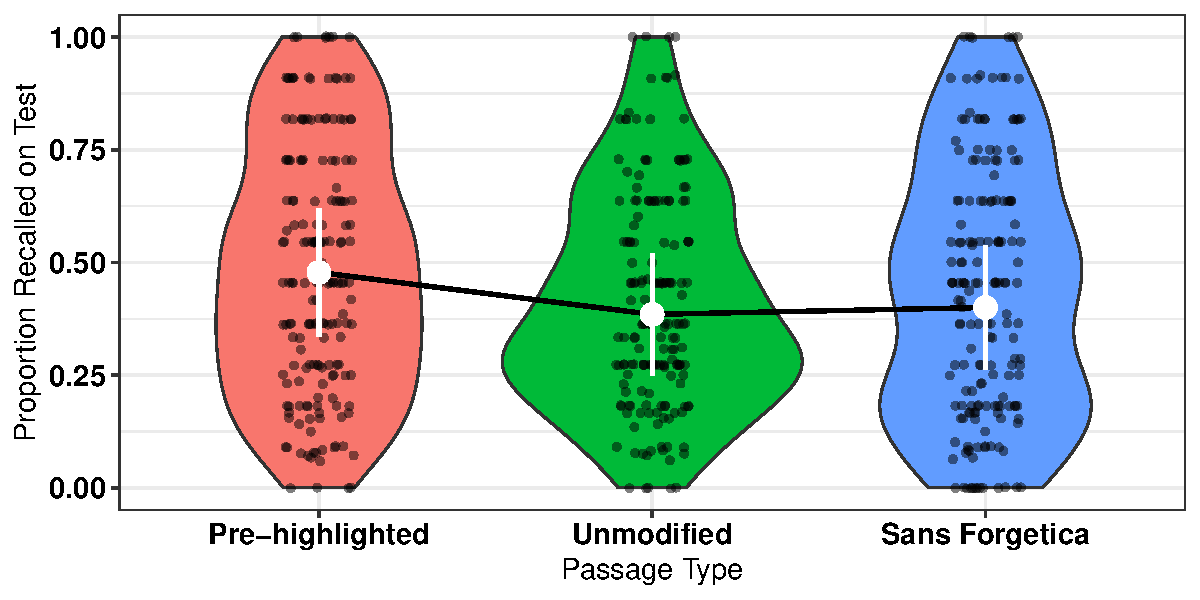
\includegraphics{SF_Paper_1_files/figure-latex/unnamed-chunk-3-1} 

}

\caption{Proportion recalled as a function of passage type. Violin plots represent the kernal density of avearge accuracy (black dots) with the mean (white dot) and 95\% CIs.}\label{fig:unnamed-chunk-3}
\end{figure}

\hypertarget{exploratory-analysis}{%
\subsubsection{Exploratory Analysis}\label{exploratory-analysis}}

In Experiment 2 we also asked students about their metacognitive awareness of the manipulations known as JOLs. To examine differences, we conducted separate independent t-tests. Looking at JOLs (see Figure 4), the unmodified passage was given higher JOLs (\emph{M} = 57.4, \emph{SD} = 25.2) than the pre-highlighted passage (\emph{M} = 50.3, \emph{SD} = 26.0), \emph{t}(525) = -2.55, \emph{SE} = 2.78, \emph{p}\textsubscript{tuk} = .030. There were no reliable differences between the pre-highlighted and Sans Forgetica (\emph{M} = 53.8, \emph{SD} = 27.0) passages, \emph{t}(525) = -1.26,\emph{SE} = 2.78, \emph{p}\textsubscript{tuk} = .415, or between the passage in Sans Forgetica and the passage presented normally, \emph{t}(525) = 1.28, \emph{SE} = 2.78, \emph{p}\textsubscript{tuk} = .406. That is, passages in Sans Forgetica typeface did not produce lower judgement of learning compared to an unmodified or pre-highlighted passage. Interestingly, individuals gave lower JOLs to pre-highlighted information compared to materials presented in a normal typeface. With a between-subjects design, it is not uncommon to observe no JOL differences between fluent and disfluent materials (Magreehan et al., 2016; Yue et al., 2013). Despite this, we did find lower JOLs for pre-highlighted information compared to unmodified information. One potential reason for pre-highlighted information receiving lower JOLs than the normal passage is that pre-highlighted information served to focus participants' attention to specific parts of the passage. Given the question (i.e., \enquote{How likely is it that you will be able to recall material from the passage you just read on a scale of 0 (not likely to recall) to 100 (likely to recall) in 5 minutes?}), participants might have thought pre-highlighting would hinder their ability to answer questions on the whole passage.

\begin{figure}

{\centering 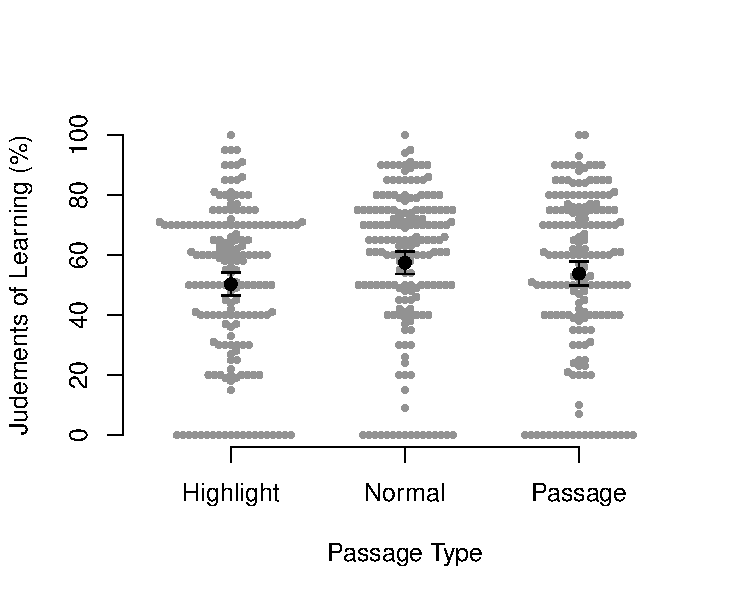
\includegraphics{SF_Paper_1_files/figure-latex/unnamed-chunk-4-1} 

}

\caption{Judgements of learning as a function of passage type. Violin plots represent the kernal density of avearge accuracy (black dots) with the mean (white dot) and 95\% CIs.}\label{fig:unnamed-chunk-4}
\end{figure}

\hypertarget{experiment-3}{%
\section{Experiment 3}\label{experiment-3}}

Both Experiments 1 and 2 utilized cued recall for the final criterion test. In previous studies, perceptual disfluency has been shown to enhance performance on yes/no recognition tests, even when there is no recall benefit (Nairne, 1988). This is thought to be because the learner is focusing on surface-level aspects during the initial perceptual identification process. This strategy should aid later recognition, but not recall, for fluent items, given that recall relies more on item elaboration than on perceptually distinctive features. In Experiment 3, we tested whether Sans Forgetica would lead to similar benefits in recognition memory. It is possible that Sans Forgetica serves to increase surface-level familiarity of a word and thus recognition, while recall is unchanged. We hypothesized no recognition memory benefit for Sans Forgetica.

\hypertarget{participants-2}{%
\subsubsection{Participants}\label{participants-2}}

Sixty participants (\emph{N} = 60) participated for partial completion of course credit. Sample size was determined by a similar procedure to the above experiments. No participants were removed for failing to meet the exclusion criteria noted above.

\hypertarget{materials-1}{%
\subsubsection{Materials}\label{materials-1}}

Stimuli were 188 single-word nouns taken from Geller et al.~(2018). All words were from the English Lexicon Project database (Balota et al., 2007). Both word frequency (all words were high frequency; mean log HAL frequency = 9.2) and length (all words were four letters) were controlled. The full set of stimuli can be found at \url{https://osf.io/dsxrc/}.

\hypertarget{design-and-procedure-1}{%
\subsubsection{Design and Procedure}\label{design-and-procedure-1}}

Disfluency (Sans Forgetica vs.~Fluent) was the single variable, manipulated within-subjects. We presented participants with 188 words, 94 at study (47 in each script condition) and 188 at test (94 old and 94 new). Words were counterbalanced across the disfluency and study/test conditions, such that each word served equally often as a target and a foil in both typefaces. The experiment was created and conducted using the Gorilla Experiment Builder {[}Anwyl-Irvine, Massonnié, Flitton, Kirkham, and Evershed (2020); \url{http://www.gorilla.sc}{]}. The experiment protocol and tasks are available to preview and copy from Gorilla Open Materials at \url{https://gorilla.sc/openmaterials/72765}. Word order was completely randomized, such that Arial and Sans Forgetica words were randomly intermixed in the study phase, and Arial and Sans Forgetica old and new words were randomly intermixed in the test phase, with old words always presented in the same script at test as they were at study.

During the study phase, a fixation cross appeared at the center of the screen for 500 ms. The fixation cross was immediately replaced by a word in the same location. To continue to the next trial, participants pressed the continue button at the bottom of the screen. Each trial was self-paced (see the General Discussion for the study time data). After the study phase, participants completed a short three-minute distractor task wherein they wrote down as many U.S. state capitals as they could. Afterward, participants took an old-new recognition test. At test, a word appeared in the center of the screen that either had been presented during study (\enquote{old}) or had not been presented during study (\enquote{new}). Old words occurred in their original script, and following the counterbalancing procedure, each new word was presented in Arial typeface or Sans Forgetica typeface. For each word presented, participants chose from one of two boxes displayed on the screen: a box labeled \enquote{old} to indicate that they had named the word during study, and a box labeled \enquote{new} to indicate they did not remember naming the word. Words stayed on the screen until participants gave an \enquote{old} or \enquote{new} response. All words were individually randomized for each participant during both the study and test phases. After the experiment, participants were debriefed.

\hypertarget{results-and-discussion-2}{%
\subsection{Results and Discussion}\label{results-and-discussion-2}}

Performance was examined with d', a memory sensitivity measure derived from signal detection theory (Macmillan \& Creelman, 2005). Hits or false alarms at ceiling or floor were changed to .99 or .01. Hits and false alarms along with sensitivity (d') can be seen in Figure 5.

Consistent with our preregistered hypothesis, there was no difference in d' between Sans Forgetica and Arial typefaces, \emph{t}(59) = 0.281, \emph{SE} = 0.05, \emph{p} = .780. There was strong evidence for no effect (BF\textsubscript{01} = 13.68).

Overall, we did not find an effect of Sans Forgetica typeface on recognition memory. This study provides further evidence that Sans Forgetica typeface is not desirable for memory, regardless of the final test format.

\begin{figure}

{\centering 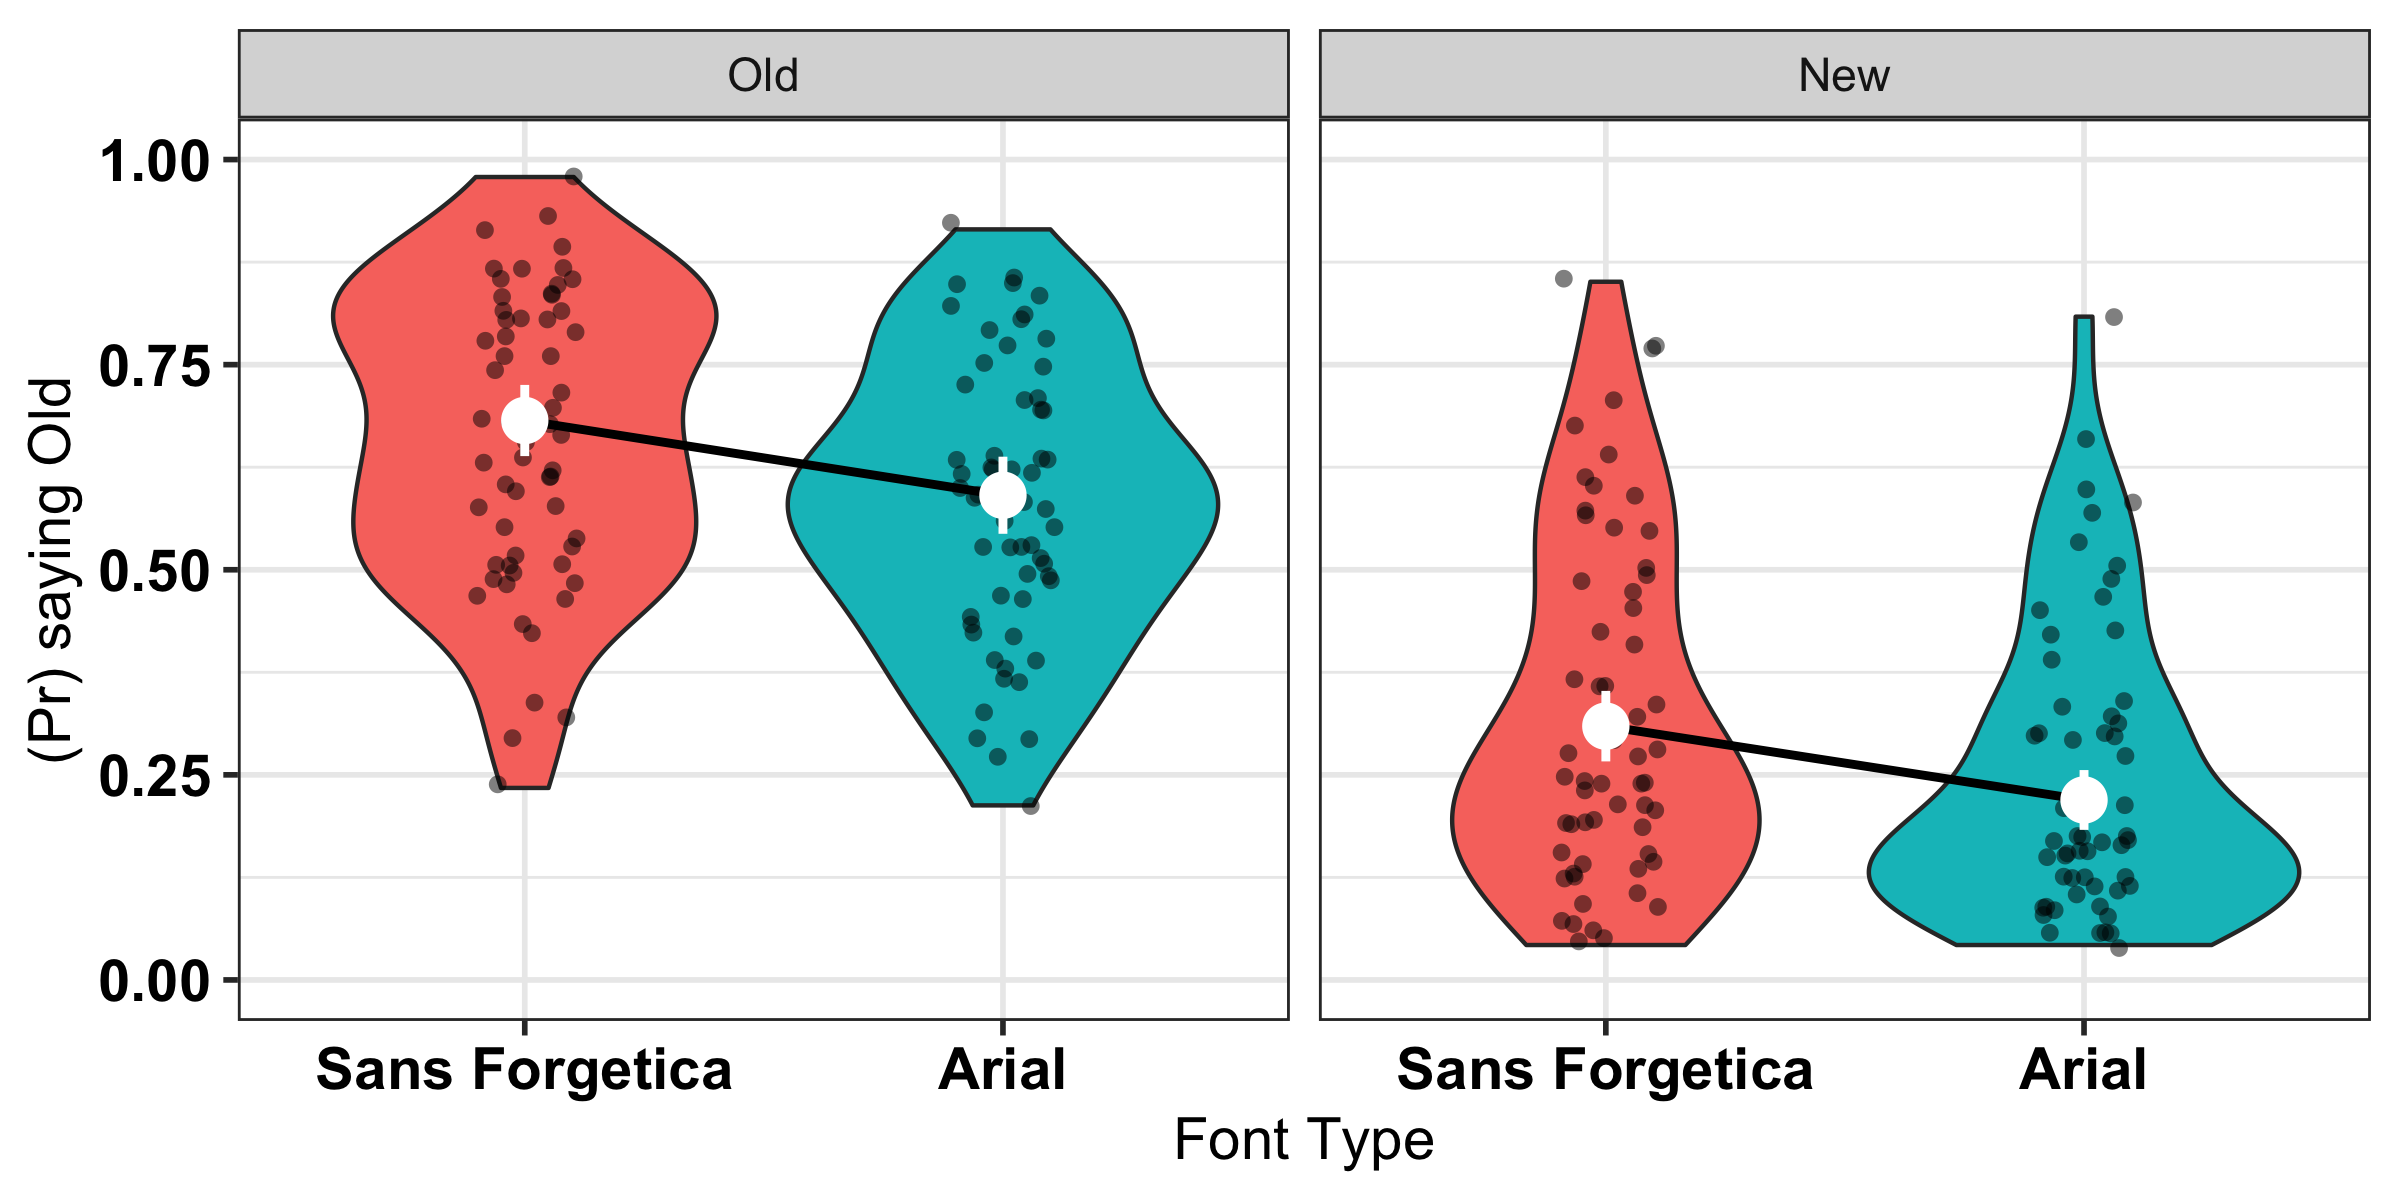
\includegraphics{SF_Paper_1_files/figure-latex/unnamed-chunk-5-1} 

}

\caption{A. Mean proportions of “old” responses. Violin plots represent the kernal density of average probability (black dots) with the mean (white dot) and within-subject 95\% CIs. B. Memory sensitivity (d'). Violin plots represent the kernal density of avearge accuracy (black dots) with the mean (white dot) and Cousineau-Morey within-subject 95\% CIs.}\label{fig:unnamed-chunk-5}
\end{figure}

\hypertarget{general-discussion}{%
\section{General Discussion}\label{general-discussion}}

The creators of the Sans Forgetica typeface as well as the media have made strong claims regarding the mnemonic benefits of Sans Forgetica. The aim of the current experiments was to test those claims empirically. In Experiment 1, Sans Forgetica typeface did not enhance memory in a cued recall task with weakly related cues. In Experiment 2, Sans Forgetica typeface did not enhance memory for a complex prose passage. In Experiment 3, Sans Forgetica typeface did not enhance recognition memory. Even with every opportunity to reveal itself, we did not find any evidence for a mnemonic benefit of Sans Forgetica typeface.

While it has been posited both in unpublished and published studies (Earp, 2018; Eskenazi \& Nix, 2020) that Sans Forgetica has a positive effect on memory, our high-powered studies with over 800 participants argue against this claim. This, along with Taylor et al. (2020) provides converging evidence that that Sans Forgetica typeface is not a desirable difficulty. Theoretically, these findings add to the literature showing that perceptual disfluency has little impact on actual memory performance (e.g., Magreehan et al., 2016; Rhodes \& Castel, 2008, p. @Rhodes2009; Rummer et al., 2016; Xie et al., 2018; Yue et al., 2013). Importantly, we did find a memory advantage for other learning techniques such as generation (Experiment 1) and pre-highlighting (Experiment 2) whose efficacy is robustly supported in the literature. That is, the conditions were ripe for a Sans Forgetica effect to emerge if it were an actual mnemonic effect.

What might account for the null effect of Sans Forgetica typeface on memory? Drawing valid conclusions about disfluency requires the use of objective disfluency measures. In many studies, perceptual disfluency is using subjective measures (e.g., JOLs or difficulty ratings), but never explicitly tested. Thus, it could be that the failure to observe an effect in the current set of studies is because Sans Forgetica typeface is simply not perceptually disfluent. Although we did not preregister explicit tests of objective disfluency, we have some preliminary evidence that Sans Forgetica is not disfluent. In Experiment 3, we collected self-paced study times for each stimulus. Self-paced study times have been used as an objective proxy for disfluency (see Carpenter \& Geller, 2020). Looking at the difference in self-paced reading times, we did not observe a significant difference between Sans Forgetica typeface (\emph{M} = 1481 ms, \emph{SD} = 1750 ms) and Arial typeface (\emph{M} = 1500 ms, \emph{SD} = 2344 ms), \emph{t}(59) = 0.469, \emph{p} = .641, BF\textsubscript{01} = 6.67. The absence of a study time disparity suggests the typeface may not be considered disfluent and could therefore explain why we did not observe an effect of Sans Forgetica typeface. It is worth noting, however, that self-paced study times might reflect variables other than, or in addition to, processing disfluency. Although self-paced study provides one way of measuring processing fluency, more precise measures of processing disfluency should be considered as well (but see Eskenazi \& Nix, 2020 for eye-tracking evidence for Sans Forgetica typeface in good spellers).

While the current set of experiments (see also Taylor et al., 2020) did not find a memory benefit for Sans Forgetica typeface, we cannot rule out that the effect might arise under different conditions. A number of boundary conditions that determine when perceptual disfluency will and will not be a desirable difficulty have been established over the past several years (see Geller et al., 2018, Geller \& Still, 2018). In the current set of experiments, we examined whether cue strength, study time, and type of test influenced whether or not we could find a mnemonic effect of Sans Forgetica on memory. We did not find any evidence that the memory benefit from Sans Forgetica is moderated by these factors. Despite this, future research should examine the role of individual difference measures (e.g., working memory capacity; Lehmann, Goussios, \& Seufert, 2016) along with other design features not tested (e.g.~test delay, testing expectancy).

\hypertarget{conclusion}{%
\subsection{Conclusion}\label{conclusion}}

Students are attracted to learning interventions that are easy to implement (Geller et al., 2018). It is no surprise, then, that Sans Forgetica has garnered so much media attention. However, in our current age of uncertainty about the quality of information, it is important to properly evaluate scientific claims made by the media, even if that information comes from widely trusted news sources. As scientists, our job is to properly evaluate the evidence and correct erroneous information. Accordingly, we are compelled to argue against the claims made by the Sans Forgetica team and various news outlets and conclude that Sans Forgetica should not be used as a learning technique to bolster learning. Our results suggest that placing material in Sans Forgetica typeface does not lead to more durable learning. It is our recommendation that students looking to remember more and forget less use learning tools such as testing or spacing that have stood the test of time.

\newpage

\hypertarget{references}{%
\section{References}\label{references}}

\begingroup
\setlength{\parindent}{-0.5in}
\setlength{\leftskip}{0.5in}

\hypertarget{refs}{}
\leavevmode\hypertarget{ref-Anwyl-Irvine2020}{}%
Anwyl-Irvine, A. L., Massonnié, J., Flitton, A., Kirkham, N., \& Evershed, J. K. (2020). Gorilla in our midst: An online behavioral experiment builder. \emph{Behavior Research Methods}, \emph{52}(1), 388--407. \url{https://doi.org/10.3758/s13428-019-01237-x}

\leavevmode\hypertarget{ref-Balota2007}{}%
Balota, D. A., Yap, M. J., Cortese, M. J., Hutchison, K. A., Kessler, B., Loftis, B., \ldots{} Treiman, R. (2007). The english lexicon project. Springer New York LLC. \url{https://doi.org/10.3758/BF03193014}

\leavevmode\hypertarget{ref-Bertsch2007}{}%
Bertsch, S., Pesta, B. J., Wiscott, R., \& McDaniel, M. A. (2007). The generation effect: A meta-analytic review. \emph{Memory and Cognition}, \emph{35}(2), 201--210. \url{https://doi.org/10.3758/BF03193441}

\leavevmode\hypertarget{ref-Bjork2011}{}%
Bjork, E. L., \& Bjork, R. A. (2011). Making things hard on yourself, but in a good way: Creating desirable difficulties to enhance learning. In \emph{Psychology and the real world: Essays illustrating fundamental contributions to society.} (pp. 56--64). New York, NY, US: Worth Publishers.

\leavevmode\hypertarget{ref-Butler2014}{}%
Butler, A. C., Marsh, E. J., Slavinsky, J. P., \& Baraniuk, R. G. (2014). Integrating Cognitive Science and Technology Improves Learning in a STEM Classroom. \emph{Educational Psychology Review}, \emph{26}(2), 331--340. \url{https://doi.org/10.1007/s10648-014-9256-4}

\leavevmode\hypertarget{ref-Carpenter2009}{}%
Carpenter, S. K. (2009). Cue Strength as a Moderator of the Testing Effect: The Benefits of Elaborative Retrieval. \emph{Journal of Experimental Psychology: Learning Memory and Cognition}, \emph{35}(6), 1563--1569. \url{https://doi.org/10.1037/a0017021}

\leavevmode\hypertarget{ref-Carpenter2006}{}%
Carpenter, S. K., Pashler, H., \& Vul, E. (2006). What types of learning are enhanced by a cued recall test? \emph{Psychonomic Bulletin and Review}, \emph{13}(5), 826--830. \url{https://doi.org/10.3758/BF03194004}

\leavevmode\hypertarget{ref-Diemand-Yauman2011}{}%
Diemand-Yauman, C., Oppenheimer, D. M., \& Vaughan, E. B. (2011). Fortune favors the: Effects of disfluency on educational outcomes. \emph{Cognition}, \emph{118}(1), 111--115. \url{https://doi.org/10.1016/j.cognition.2010.09.012}

\leavevmode\hypertarget{ref-Earp2018}{}%
Earp, J. (2018). Q\&A: Designing a font to help students remember key information.

\leavevmode\hypertarget{ref-Fowler1974}{}%
Fowler, R. L., \& Barker, A. S. (1974). Effectiveness of highlighting for retention of text material. \emph{Journal of Applied Psychology}, \emph{59}(3), 358--364. \url{https://doi.org/10.1037/h0036750}

\leavevmode\hypertarget{ref-cogsci18-Geller}{}%
Geller, J., \& Still, M. L. (2018). Testing expectancy, but not judgements of learning, moderate the disfluency effect. In J. Z. Chuck Kalish Martina Rau \& T. Rogers (Eds.), \emph{CogSci 2018} (pp. 1705--1710).

\leavevmode\hypertarget{ref-Geller2018}{}%
Geller, J., Still, M. L., Dark, V. J., \& Carpenter, S. K. (2018). Would disfluency by any other name still be disfluent? Examining the disfluency effect with cursive handwriting. \emph{Memory and Cognition}, \emph{46}(7), 1109--1126. \url{https://doi.org/10.3758/s13421-018-0824-6}

\leavevmode\hypertarget{ref-Kornell2016}{}%
Kornell, N., \& Vaughn, K. E. (2016). How Retrieval Attempts Affect Learning: A Review and Synthesis. \emph{Psychology of Learning and Motivation - Advances in Research and Theory}, \emph{65}, 183--215. \url{https://doi.org/10.1016/bs.plm.2016.03.003}

\leavevmode\hypertarget{ref-Lakens2014}{}%
Lakens, D., \& Evers, E. R. K. (2014). Sailing From the Seas of Chaos Into the Corridor of Stability: Practical Recommendations to Increase the Informational Value of Studies. \emph{Perspectives on Psychological Science : A Journal of the Association for Psychological Science}, \emph{9}(3), 278--292. \url{https://doi.org/10.1177/1745691614528520}

\leavevmode\hypertarget{ref-Lehmann2016}{}%
Lehmann, J., Goussios, C., \& Seufert, T. (2016). Working memory capacity and disfluency effect: an aptitude-treatment-interaction study. \emph{Metacognition and Learning}, \emph{11}(1), 89--105. \url{https://doi.org/10.1007/s11409-015-9149-z}

\leavevmode\hypertarget{ref-Macmillan2005}{}%
Macmillan, N. A., \& Creelman, C. D. (2005). \emph{Detection theory: A user's guide, 2nd ed.} (pp. xix, 492--xix, 492). Mahwah, NJ, US: Lawrence Erlbaum Associates Publishers.

\leavevmode\hypertarget{ref-Magreehan2016}{}%
Magreehan, D. A., Serra, M. J., Schwartz, N. H., \& Narciss, S. (2016). Further boundary conditions for the effects of perceptual disfluency on judgments of learning. \emph{Metacognition and Learning}, \emph{11}(1), 35--56. \url{https://doi.org/10.1007/s11409-015-9147-1}

\leavevmode\hypertarget{ref-Mulligan1996}{}%
Mulligan, N. W. (1996). The effects of perceptual interference at encoding on implicit memory, explicit memory, and memory for source. \emph{Journal of Experimental Psychology: Learning Memory and Cognition}, \emph{22}(5), 1067--1087. \url{https://doi.org/10.1037/0278-7393.22.5.1067}

\leavevmode\hypertarget{ref-Nairne1988}{}%
Nairne, J. S. (1988). The Mnemonic Value of Perceptual Identification. \emph{Journal of Experimental Psychology: Learning, Memory, and Cognition}, \emph{14}(2), 248--255. \url{https://doi.org/10.1037/0278-7393.14.2.248}

\leavevmode\hypertarget{ref-Rhodes2008}{}%
Rhodes, M. G., \& Castel, A. D. (2008). Memory Predictions Are Influenced by Perceptual Information: Evidence for Metacognitive Illusions. \emph{Journal of Experimental Psychology: General}, \emph{137}(4), 615--625. \url{https://doi.org/10.1037/a0013684}

\leavevmode\hypertarget{ref-Rhodes2009}{}%
Rhodes, M. G., \& Castel, A. D. (2009). Metacognitive illusions for auditory information: Effects on monitoring and control. \emph{Psychonomic Bulletin and Review}, \emph{16}(3), 550--554. \url{https://doi.org/10.3758/PBR.16.3.550}

\leavevmode\hypertarget{ref-Rosner2015}{}%
Rosner, T. M., Davis, H., \& Milliken, B. (2015). Perceptual blurring and recognition memory: A desirable difficulty effect revealed. \emph{Acta Psychologica}, \emph{160}, 11--22. \url{https://doi.org/10.1016/j.actpsy.2015.06.006}

\leavevmode\hypertarget{ref-Rummer2016}{}%
Rummer, R., Schweppe, J., \& Schwede, A. (2016). Fortune is fickle: null-effects of disfluency on learning outcomes. \emph{Metacognition and Learning}, \emph{11}(1), 57--70. \url{https://doi.org/10.1007/s11409-015-9151-5}

\leavevmode\hypertarget{ref-Silvers1997}{}%
Silvers, V. L., \& Kreiner, D. S. (1997). The effects of pre-existing inappropriate highlighting onreading comprehension. \emph{Reading Research and Instruction}, \emph{36}(3), 217--223. \url{https://doi.org/10.1080/19388079709558240}

\leavevmode\hypertarget{ref-Slamecka1978}{}%
Slamecka, N. J., \& Graf, P. (1978). The generation effect: Delineation of a phenomenon. \emph{Journal of Experimental Psychology: Human Learning \& Memory}, \emph{4}(6), 592--604. \url{https://doi.org/10.1037/0278-7393.4.6.592}

\leavevmode\hypertarget{ref-Sungkhasettee2011}{}%
Sungkhasettee, V. W., Friedman, M. C., \& Castel, A. D. (2011). Memory and metamemory for inverted words: Illusions of competency and desirable difficulties. \emph{Psychonomic Bulletin and Review}, \emph{18}(5), 973--978. \url{https://doi.org/10.3758/s13423-011-0114-9}

\leavevmode\hypertarget{ref-Taylor2020}{}%
Taylor, A., Sanson, M., Burnell, R., Wade, K. A., \& Garry, M. (2020). Disfluent difficulties are not desirable difficulties: the (lack of) effect of Sans Forgetica on memory. \emph{Memory}, 1--8. \url{https://doi.org/10.1080/09658211.2020.1758726}

\leavevmode\hypertarget{ref-Westfall2016}{}%
Westfall, J. (2016). \emph{PANGEA: Power ANalysis for GEneral Anova designs}. Retrieved from \url{http://jakewestfall.org/pangea/}

\leavevmode\hypertarget{ref-Xie2018}{}%
Xie, H., Zhou, Z., \& Liu, Q. (2018). Null Effects of Perceptual Disfluency on Learning Outcomes in a Text-Based Educational Context: a Meta-analysis. \emph{Educational Psychology Review}, \emph{30}(3), 745--771. \url{https://doi.org/10.1007/s10648-018-9442-x}

\leavevmode\hypertarget{ref-Yue2013}{}%
Yue, C. L., Castel, A. D., \& Bjork, R. A. (2013). When disfluency is-and is not-a desirable difficulty: The influence of typeface clarity on metacognitive judgments and memory. \emph{Memory and Cognition}, \emph{41}(2), 229--241. \url{https://doi.org/10.3758/s13421-012-0255-8}

\endgroup

\end{document}
